%%===========================================================%%
%%                                                           %%
%%                          INTRODUCTION                          %%
%%                                                           %%
%%===========================================================%%


\chapter{Introduction}\label{chap:introduction}

\section{Diffractive interactions in $pp$ collisions}
Diffractive processes at high energies are characterized by the exchange of the Pomeron, a color singlet object with quantum numbers of the vacuum described by the Regge theory \cite{barone}\cite{donnachie_dosch_landshoff_nachtmann_2002}. Due to non-perturbative nature of interactions, there are difficulties in applying QCD to diffraction. Experimentally, diffraction is identified as interaction with large rapidity gap, i.e. final states are separated in rapidity space.

There are two processes of interest, shown in Figure \ref{fig:sdcdgraph} (a, b), the Central $\left(\textnormal{CD: }p+p\to p+X+p\right)$ and Single $\left(\textnormal{SD: }p+p\to p+X\right)$ Diffractive scattering, where $X$ is the diffractive system. In CD interactions, two protons stay intact after the scattering, whereas in SD only one proton.
\begin{figure}[hb]
	\centering
	\parbox{0.484\textwidth}{
		\centering
		\begin{subfigure}[b]{\linewidth}{
				\subcaptionbox{\label{fig:cdgraph}}{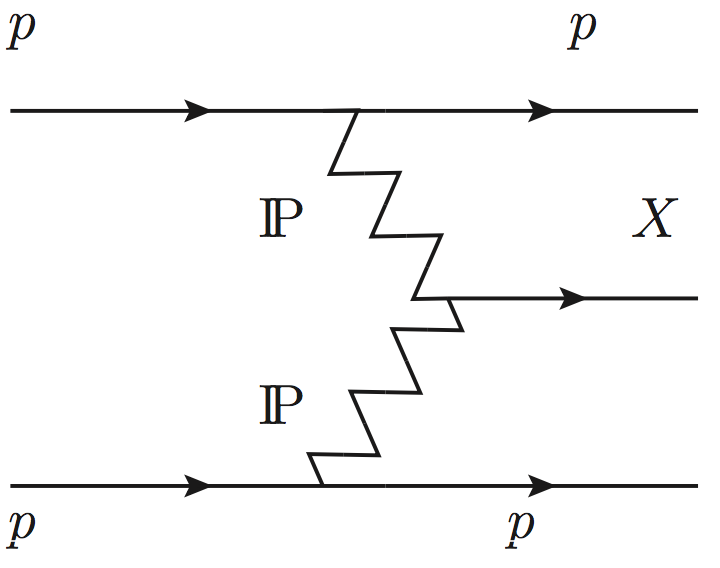
\includegraphics[width=\linewidth]{graphics/introduction/cd.png}}}
		\end{subfigure}
	}
	\quad
	\parbox{0.484\textwidth}{
		\centering
		\begin{subfigure}[b]{\linewidth}{
				\subcaptionbox{\label{fig:sdgraph}}{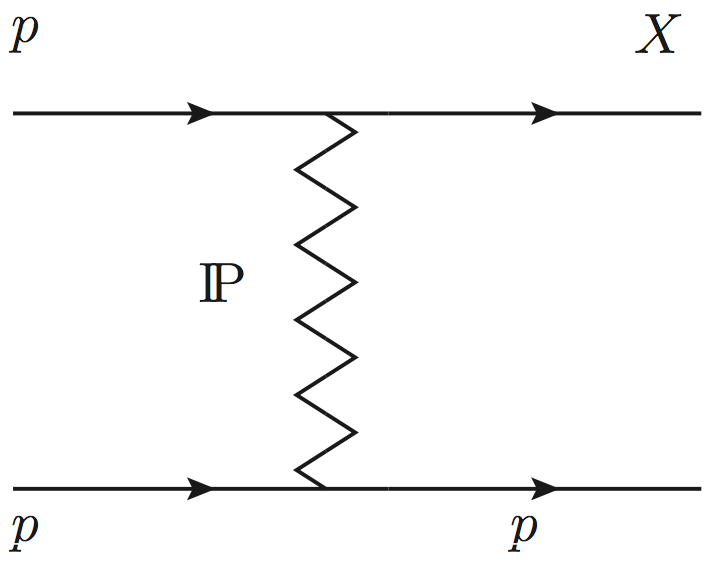
\includegraphics[width=\linewidth]{graphics/introduction/sd.png}}}
		\end{subfigure}
	}%
	\caption[Diagrams of Central Diffraction and Single Diffraction]{Diagrams of Central Diffraction (a) and Single Diffraction (b).}
	 \label{fig:sdcdgraph}
\end{figure}
The (identified) charged particle production in the mid-rapidity region has been widely studied in minimum bias inelastic hadron-hadron collisions starting from the very first experiments performed at ISR at CERN throughout contemporary measurements with very high center-of-mass energy at RHIC \cite{systmeasurhic} and LHC \cite{Adam:2015qaa}. This is the first measurement with tagged forward protons, 
which allows efficient identification of diffractive events. The measured particle spectra and ratios deliver information on collision dynamics, mechanism and allows to validate some phenomenological models and tune some general purpose MC generators.
\section{Baryon number transfer}
In the Standard Model the baryon 
number is conserved in all interactions. The conserved baryon number associated with the beam particles is called "baryon number transfer" and has been studied theoretically for some time~\cite{Kopeliovich:1988qm,Rossi:1977cy,Bopp:2000cr}. The baryon number transfer, which is quantified by the baryon to anti-baryon ratios, is often described as a function of the size of the transport in rapidity represented by
rapidy difference $\Delta y = y_{beam}-y$, where $y_{beam}=\ln\left(\sqrt{s}/m_p\right)$ is the rapidity of the beam and $y$ the rapidity of the particles produced in the central system. In~the~String Junction Model  \cite{Rossi:1977cy} the baryon number can be transferred over large distances in the rapidity. In this picture, baryon number transfer is exponentially suppressed as a function of the rapidity interval $\Delta y$. In particular, when there are only purely gluonic exchanges between the valence quarks of the proton, the baryon number transfer does not depend on the rapidity and approaches a constant and finite value~\cite{Kopeliovich:1988qm}. There is also a model \cite{Bopp:2000cr}, in which the initial baryon may end up at the backward end of the diffractive system. The~edge of the rapidity gap $\Delta\eta$ is related to the~relative proton momentum loss $\xi=\Delta E/E$, $\Delta\eta\approx-\ln\xi=-\ln\left(M_X^2/s\right)$. %Therefore, the measurement of particle ratios as a function of $\xi$ of the outgoing protons should be taken into account to validate this model. 
There is a large number of the experimental data available on baryon number transfer \cite{Aamodt:2010dx}. The mid-rapidity  anti-proton to proton ratio is sensitive to center-of-mass energy  and varies between $0.4$ for ISR energies and almost $1$ for the~LHC, where the~transfer size in the rapidity space $\Delta y$ is large and equals to almost $9$ units. In addition, this effect was also measured by the H1 Collaboration in proton-photon interactions \cite{Kopeliovich:1998ps}, where the data show that there is a sizeable baryon to anti-baryon asymmetry. The similar effect can be studied in SD interactions, where the direction of the initial baryon is uniquely defined.

%---------------------------

%---------------------------
